% =========================================================================
\documentclass[aspectratio=1610]{beamer}
%\documentclass[aspectratio=1610]{beamer}

% ========================= Theme =========================================
\usetheme{Berkeley}
\usecolortheme{seahorse}

% ========================= Essential packages ============================
%\usepackage{hyperref}
%\hypersetup{
%    colorlinks = true,
%    linkcolor = blue,
%    citecolor = blue,
%    filecolor = blue,
%    urlcolor = blue
%}

% ========================= Frame notes systm ============================
%\usepackage{pgfpages}
%\setbeameroption{show notes on second screen}

% ========================= Plotting ======================================
\usepackage{calc}
\usepackage{tikz}
\usetikzlibrary{arrows,
                arrows.meta,
                calc,
                chains,
                quotes,
                positioning,
                shapes,
                shapes.geometric}
\usepackage{graphicx}
\usepackage{graphics}
\usepackage{pgfplots}
\pgfplotsset{width=7cm,compat=1.17}

%% ============================== Tabular =================================
\usepackage{booktabs}
\usepackage{tabularx,ragged2e}
\usepackage{array}
\usepackage{multirow}
\usepackage{siunitx}
  \sisetup{detect-all}
\usepackage{adjustbox}
\usepackage{rotating}
\usepackage{threeparttable}
\usepackage[justification=centering]{caption}

%% ============================== Text boxes ==============================
\usepackage[most]{tcolorbox}

%% ========================== Coding snippets =============================
% Default fixed font does not support bold face
%\usepackage{minted}
%\usemintedstyle{vs}

% ========================= Infor on authors ==============================
\title[Visualization Design]%
{Visualization Design}
\subtitle{Design Principles and Main Visual Forms}
\author{S.~Santoni\inst{1}}
\institute{
	\inst{1}%
	Bayes Business School
	}
\date{MSc in Business Analytics, 2024/25}

% ============================ Colors =====================================
\definecolor{base_c}{rgb}{0.6,0,0}
\definecolor{comp_c}{rgb}{0.09803921568627451, 0.6901960784313725, 0.7529411764705882}
\definecolor{tri_1}{rgb}{0.09803921568627451, 0.7686274509803922, 0.19215686274509805}
\definecolor{tri_2}{rgb}{0.19215686274509805, 0.09803921568627451, 0.7686274509803922}

% ========================= TOC  ==========================================
\AtBeginSection[]
{
	\begin{frame}
		       \frametitle{Outline}
		       \tableofcontents[currentsection,currentsubsection]
	\end{frame}
}

% ========================= References ===================================
\usepackage[style=numeric,backend=biber]{biblatex}
\addbibresource{bibliography.bib}

% =========================== TOC =========================================
\AtBeginSubsection[]
{
    \begin{frame}
        \frametitle{Outline}
        \tableofcontents[currentsection,currentsubsection]
    \end{frame}
}

% ========================= Document  ====================================
\begin{document}

\begin{frame}
	\titlepage
\end{frame}

\begin{frame}{Outline}
	\tableofcontents
\end{frame}

% ========================== Graphical excellence ========================
\section{Graphical Excellence}

\begin{frame}
	\frametitle{What is Good Data Viz?}
	\begin{figure}
		\begin{small}
			\begin{center}
				\includegraphics[width=0.95\textwidth]{images/subjectivity.jpg}
			\end{center}
		\end{small}
	\end{figure}
\end{frame}

\begin{frame}
	\frametitle{Example A: A Plot from the a Towards Data Science Post}
	\begin{figure}
		\begin{small}
			\begin{center}
				\includegraphics[width=0.9\textwidth]{images/plotly_scatter.png}
			\end{center}
		\end{small}
	\end{figure}

	\vspace{-1em}

	\footnotesize
	Source: \href{https://towardsdatascience.com/enhance-your-plotly-express-scatter-plot-with-marginal-plots-de469d42f12a}
	{https://towardsdatascience.com/enhance-your-plotly...}
\end{frame}

\begin{frame}
	\frametitle{Example B: A Chart from an Article in The Economist}
	\begin{figure}
		\begin{small}
			\begin{center}
				\includegraphics[width=0.75\textwidth]{images/economist_scatter.png}
			\end{center}
		\end{small}
	\end{figure}

	\footnotesize
	Source: \href{https://www.economist.com/united-states/2015/03/12/it-depends-what-you-study-not-where}
	{https://www.economist.com/...it-depends-what-you-study-not-where}
\end{frame}

\begin{frame}
	\frametitle{Graphical Excellence according to Tufte}
	Per Tufte's work \cite{tufte2001}, excellence in statistical graphs consists of complex
	\emph{``ideas communicated with clarity, precision, and
		efficiency.''}

	\vspace{1em}

	Graphical displays pursuing clarity, precision, and efficiency \emph{``
		give to the viewer the greatest number of ideas
		in the shortest time with the least ink in the smallest space.''}

	\begin{figure}
		\begin{small}
			\begin{center}
				\includegraphics[width=0.75\textwidth]{
					images/graphical_excellence.png
				}
			\end{center}
		\end{small}
	\end{figure}

\end{frame}

\begin{frame}
	\frametitle{How to Reach Clarity, Efficiency, and Precision?}
	Tufte points out graphical displays should
	\begin{itemize}
		\item
		      Show the data
		\item
		      Induce the viewer to think about the substance rather than
		      about the methodology, graphical design, the technology of
		      graphic production, or something else
		\item
		      Avoid distorting what the data have to say
		\item
		      Present many numbers in a small space
		\item
		      Make large datasets coherent
		\item
		      Encourage the eye to compare different pieces of data
		\item
		      Reveal the data at several levels of detail, from a broad
		      overview to the fine structure
		\item
		      Serve a reasonably clear purpose: description,
		      exploration, tabulation, or decoration
		\item
		      Be closely intergrated with the statistical and verbal
		      description of a data set
	\end{itemize}
\end{frame}

\begin{frame}
	\frametitle{Show the Data!}
	Here is a classic example on the importance of showing the data,
	the case of Anscombe's quartet \cite{anscombe1973}.

	\begin{figure}
		\begin{small}
			\begin{center}
				\includegraphics[width=1\textwidth]{
					images/anscombe_i.png
				}
			\end{center}
		\end{small}
	\end{figure}
	\footnote{See \cite[][page 14]{tufte2001}}
\end{frame}

\begin{frame}
	\frametitle{Show the Data! (cont'd)}
	\begin{figure}
		\begin{small}
			\begin{center}
				\includegraphics[width=0.80\textwidth]{
					images/anscombe_ii.png
				}
			\end{center}
		\end{small}
	\end{figure}

\end{frame}
% ============================ Graphical integrity =========================
\section{Graphical Integrity}

\begin{frame}
	\frametitle{Excellent Graphical Displays Tell the Truth!}
	%\subtitle{A time series plot example}
	\begin{columns}
		\begin{column}{0.5\textwidth}
			\begin{figure}
				\begin{small}
					\begin{center}
						\includegraphics[width=0.9\textwidth]{
							images/commission_to_agents.png
						}
					\end{center}
				\end{small}
			\end{figure}
		\end{column}
		\begin{column}{0.5\textwidth}
			Tufte \cite[][page 54]{tufte2001} observes
			that \emph{`the pseudo-decline was created by comparing six months' worth of
				payments in 1978 to a full year's worth in 1976 and 1977, with the
				lie repeated four times.''}
		\end{column}
	\end{columns}
	\footnotesize
	Source: New York Times, August 8, 1978, page D-1.
\end{frame}

\begin{frame}
	\frametitle{Excellent Graphical Displays Tell the Truth!}
	%\subtitle{An infographic example}
	\begin{figure}
		\begin{small}
			\begin{center}
				\includegraphics[width=0.95\textwidth]{
					images/fuel_economy.png}
			\end{center}
		\end{small}
	\end{figure}

	\footnotesize
	Source: New York Times, August 9, 1978, page D-2.
\end{frame}

\begin{frame}
	\frametitle{The Lie Factor}
	\begin{columns}
		\begin{column}{0.5\textwidth}
			\footnotesize
			\begin{equation}
				\text{Lie Factor} = \frac{\text{Size of the effect shown in graphic}}
				{\text{Size of effect in data}}
			\end{equation}
		\end{column}
		\begin{column}{0.5\textwidth}
			\begin{figure}
				\begin{small}
					\begin{center}
						\includegraphics[width=0.95\textwidth]{
							images/is_that_correct.png}
					\end{center}
				\end{small}
			\end{figure}
		\end{column}
	\end{columns}
\end{frame}

\begin{frame}
	\frametitle{The Lie Factor}
	\begin{columns}
		\begin{column}{0.5\textwidth}
			\footnotesize
			Effec size in data

			\begin{equation}
				\frac{27.5 - 18.0}{18.0} = 5.3
			\end{equation}

			\vspace{1em}

			Effect shown in graphic

			\begin{equation}
				\frac{5.3 - 0.6}{0.6} = 78.3
			\end{equation}

			\vspace{1em}

			Lie factor

			\begin{equation}
				\frac{78.3}{5.3} = 14.8
			\end{equation}
		\end{column}
		\begin{column}{0.5\textwidth}
			\begin{figure}
				\begin{small}
					\begin{center}
						\includegraphics[width=0.95\textwidth]{
							images/fuel_economy.png
						}
					\end{center}
				\end{small}
			\end{figure}
		\end{column}
	\end{columns}
\end{frame}

\begin{frame}
	\frametitle{Let Us Redesign the `Fuel Econmy Standards' Graph}

	Tufte points out \emph{``it is easy enough to decorate the data
		without lying''}
	\begin{figure}
		\begin{small}
			\begin{center}
				\includegraphics[width=0.4\textwidth]{
					images/redo_fuel_economy.png
				}
			\end{center}
		\end{small}
	\end{figure}

\end{frame}

\begin{frame}
	\frametitle{Another Time Series that Lies}
	\begin{figure}
		\begin{small}
			\begin{center}
				\includegraphics[width=0.7\textwidth]{
					images/nsf.png
				}
			\end{center}
		\end{small}
	\end{figure}

	\footnotesize
	Source: National Science Foundation, Science Indicators, 1974.

\end{frame}


\begin{frame}
	\frametitle{Yet another Time Series that Lies}
	\begin{figure}
		\begin{small}
			\begin{center}
				\includegraphics[width=0.7\textwidth]{
					images/nys_budget.png
				}
			\end{center}
		\end{small}
	\end{figure}

	\footnotesize
	Source: New York Times, February 1, 1976, page IV-6.
\end{frame}

\begin{frame}
	\frametitle{Yet another Time Series that Lies}
	\begin{figure}
		\begin{small}
			\begin{center}
				\includegraphics[width=1\textwidth]{
					images/errors.png
				}
			\end{center}
		\end{small}
	\end{figure}
\end{frame}

\begin{frame}
	\frametitle{Chartjunks Distort the Data!}
	\begin{figure}
		\begin{small}
			\begin{center}
				\includegraphics[width=1\textwidth]{
					images/errors_.png
				}
			\end{center}
		\end{small}
	\end{figure}
\end{frame}

\begin{frame}
	\frametitle{Let Us Redesign the `NYS Total Budget Expenditures' Graph}
	\begin{figure}
		\begin{small}
			\begin{center}
				\includegraphics[width=0.8\textwidth]{
					images/redo_nys_budget.png
				}
			\end{center}
		\end{small}
	\end{figure}
\end{frame}

\begin{frame}
	\frametitle{How Can Graphic Mediocrity Be Remedied?}
	Graphical competence demands three different skills

	\begin{itemize}
		\item Substantive skills
		\item Statistical skills
		\item Design skills
	\end{itemize}
\end{frame}

\begin{frame}
	\frametitle{Let Us Redesign the `NYS Total Budget Expenditures' Graph}
	\begin{figure}
		\begin{small}
			\begin{center}
				\includegraphics[width=0.8\textwidth]{
					images/redo_nys_budget.png
				}
			\end{center}
		\end{small}
	\end{figure}
\end{frame}

% =========================== Design principles ============================
\section{Design Principles}

\begin{frame}{The Data Visualization Process acccording to Cairo}
	{Data, information, knowledge, wisdom}{}
	\begin{figure}
		\includegraphics[width=0.95\textwidth]{images/cairo_model.png}
		\caption*{Source is \cite[][page 29]{cairo2012}}
	\end{figure}
\end{frame}

\begin{frame}{How to Navigate the Data Visualization Process?}{}
	\begin{columns}
		\begin{column}{0.5\textwidth}
			\begin{figure}
				\includegraphics[width=0.95\textwidth]
				{images/edward-tufte.jpeg}
			\end{figure}
		\end{column}
		\begin{column}{0.5\textwidth}
			Tufte \cite[][page 92]{tufte2001} suggests to adhere to a
			basic design principle:

			\begin{quote}

				\vspace{1em}


				Show the data.

				\vspace{1em}

				The principle is the basis for a theory
				for a theory of data graphics.
			\end{quote}
		\end{column}
	\end{columns}
\end{frame}

\begin{frame}{}{}
	\LARGE \centering Fine --- So What?!
\end{frame}

\begin{frame}{Maximize the Data-Ink Ratio!!}{}
	\begin{center}
		\begin{equation*}
			\text{Data-Ink ratio} = \frac{
				\text{data-ink}
			}
			{
				\text{total ink used to print the graphic design}
			}
		\end{equation*}
	\end{center}

	\vspace{2em}

	\textbf{Data-ink} is the non-erasable core of a graphic, the
	non-redundant ink arranged in response to variation in the numbers
	represented.
\end{frame}

\begin{frame}{Theee Versions of the Same Scatter Diagram}
	{Low data-ink ratio}
	\begin{figure}
		\begin{center}
			\includegraphics[width=0.55\textwidth]{images/low.png}
		\end{center}
	\end{figure}
\end{frame}

\begin{frame}{Theee Versions of the Same Scatter Diagram}
	{Substantial data-ink ratio}
	\begin{figure}
		\begin{center}
			\includegraphics[width=0.6\textwidth]{images/high.png}
		\end{center}
	\end{figure}
\end{frame}

\begin{frame}{Theee Versions of the Same Scatter Diagram}
	{Null data-ink ratio}
	\begin{figure}
		\begin{center}
			\includegraphics[width=0.5\textwidth]{images/null.png}
		\end{center}
	\end{figure}
\end{frame}

\begin{frame}{How to Improve the Data-Ink Ratio?}
	\begin{columns}[t]
		\begin{column}{0.5\textwidth}
			\begin{center}
				\textbf{Pre-chart execution:\\careful scoping}
			\end{center}
			\small
			\pause
			\begin{tcolorbox}[
					colback=blue!5!white,
					colframe=blue!60!black,
					title={
							\centering
							!! Maximize the data-ink ratio !!
						}]
				\raggedright Every bit of ink on a graphic requires a reason
				--- and the reason should be that the ink presents
				new information.
			\end{tcolorbox}

		\end{column}
		\pause
		\begin{column}{0.5\textwidth}
			\begin{center}
				\textbf{Post-chart execution:\\critical assessment}
			\end{center}
			\pause
			\small
			\begin{tcolorbox}[
					colback=blue!5!white,
					colframe=blue!60!green,
					title={
							\centering
							!! Erase the non data-ink !!
						}]
				\raggedright Non data-ink data clutters up the data, as is the case
				of a thick mesh of grid lines, or gratuitious
				decorations.
			\end{tcolorbox}

			\pause

			\begin{tcolorbox}[
					colback=blue!5!white,
					colframe=blue!60!green,
					title={
							\centering
							!! Erase redundant data-ink !!
						}]
				\raggedright Bilateral symmetry of data meausures also creates
				redundancy as in the box plot and the open bar.
			\end{tcolorbox}

		\end{column}
	\end{columns}
\end{frame}

% ========================== Chartjunk - not to do =========================

\section{Chartjunks --- How Not To Design a Chart}

\begin{frame}{Chartjunk? Give me a Break!!}{}
	\begin{quote}
		\textit
		``The interior decoration of graphics generates a lot of ink that not thell the
		viewer anything new. The purpose of decoration varies — to make the graphic
		appear more scientific and precise, to enliven the display, to give the designer
		an opportunity to exercise artistics skills. Regardless of its cause, it is all
		non data-data-ink or redundant data-ink, and it is often chartjunk.''
	\end{quote}

	\raggedleft --- Source is \cite[][page 107]{tufte2001}
\end{frame}

\begin{frame}
	{Moir\'e Effects}
	{...geometric shapes creating a sense of movement}
	\begin{figure}
		\begin{center}
			\includegraphics[width=0.7\textwidth]
			{images/moire_effects.png}
		\end{center}
	\end{figure}
\end{frame}

\begin{frame}
	{Get Rid of Moir\'e Effects}
	{Example 1 --- Source is ``Instituto de Expansao Commercial (1929)''}
	\centering
	\begin{figure}
		\includegraphics[width=0.7\textwidth]{images/moire_effect_1.png}
	\end{figure}
\end{frame}

\begin{frame}
	{Get Rid of Moir\'e Effects}
	{Example 2 --- Source is``Kouchoukos et al. (1994), New England Journal of Medicine''}
	\centering
	\begin{figure}
		\includegraphics[width=0.7\textwidth]{images/moire_effect_2.png}
	\end{figure}
\end{frame}

\begin{frame}
	{Get Rid of Moir\'e Effects}
	{Example 3 --- Source is ``JASA style sheet (1976), Journal of the American Statistical Association''}
	\centering
	\begin{figure}
		\includegraphics[width=0.6\textwidth]{images/moire_effect_3.png}
	\end{figure}
\end{frame}

\begin{frame}
	{Use Grids Conscientiously}
	{Example --- Source is ``Institut National de la Statistique et des
		\'Etudes \'Economiques''}
	\centering
	\begin{figure}
		\includegraphics[width=0.6\textwidth]{images/grid_1.png}
	\end{figure}
\end{frame}

\begin{frame}
	{Use Grids Conscientiously}
	{Redesigning the previous example}
	\centering
	\begin{figure}
		\includegraphics[width=0.5\textwidth]{images/grid_2.png}
	\end{figure}
\end{frame}

\begin{frame}{Have You Created a `Duck Chart'?}{\textit{Big Duck}, Flanders,
		New York, photograph by Edward Tufte, July 2000.}
	\begin{figure}
		\begin{center}
			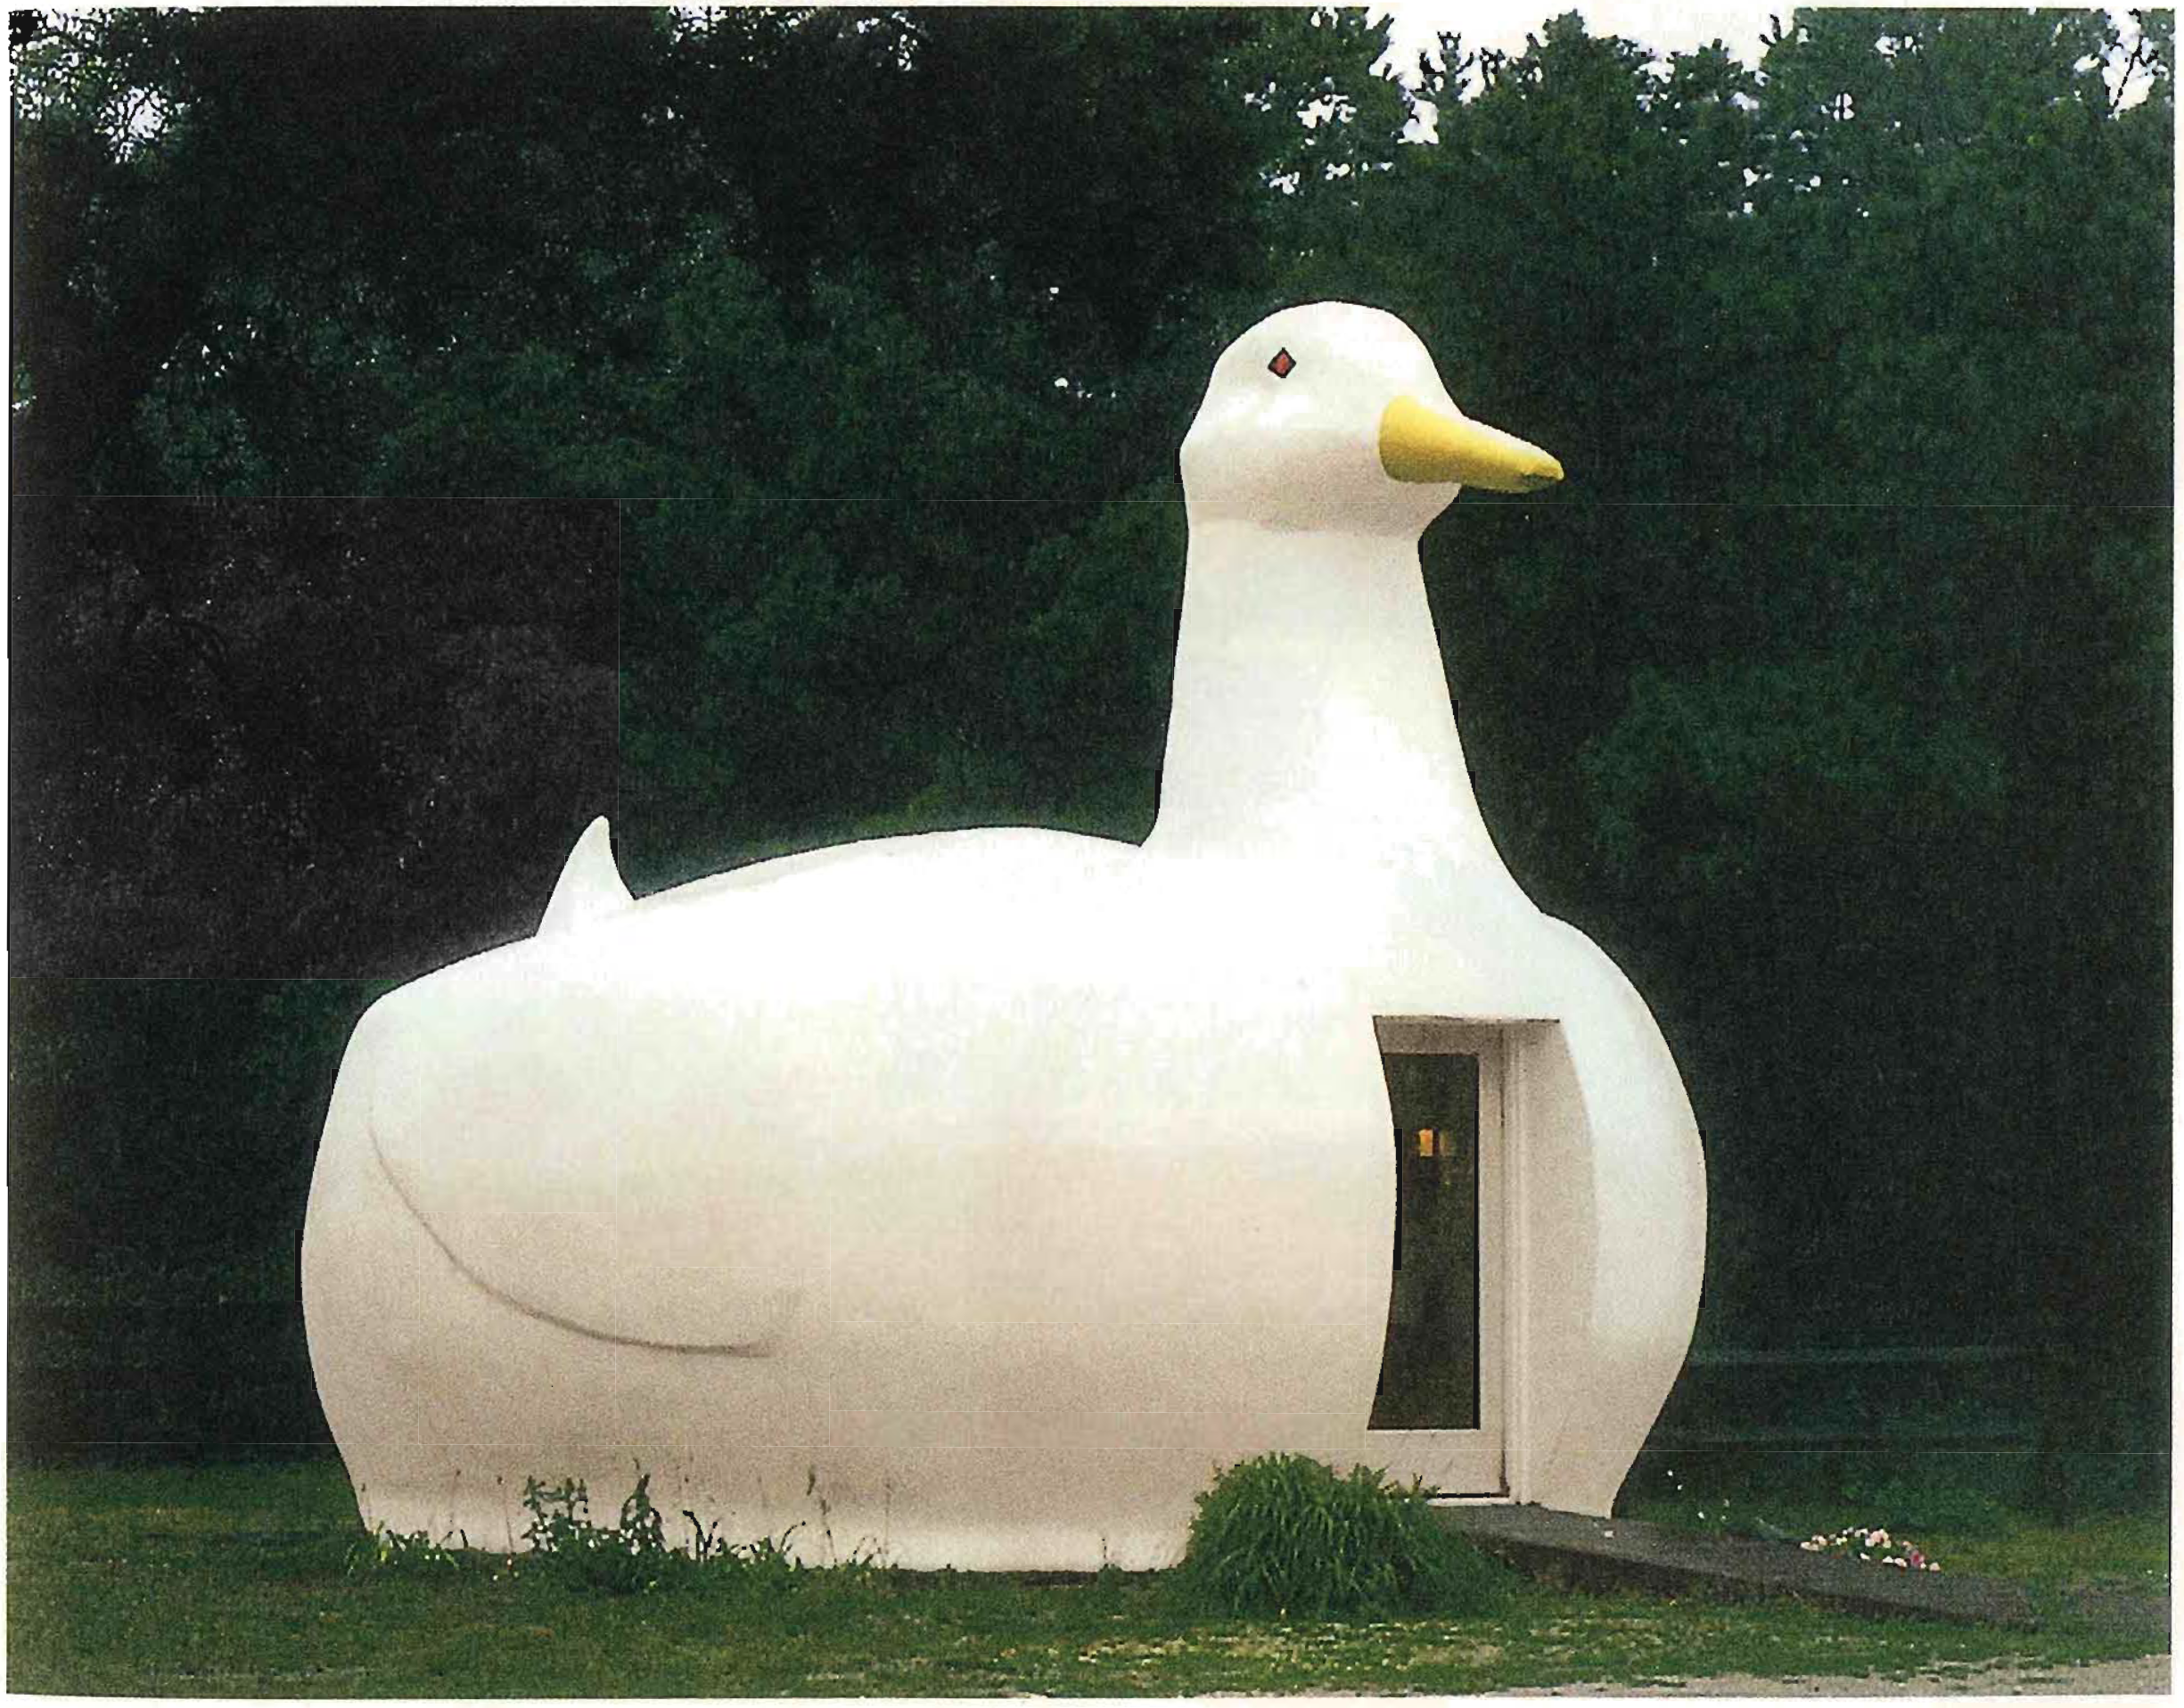
\includegraphics[width=0.7\textwidth]{images/big_duck.png}
		\end{center}
	\end{figure}
\end{frame}

\begin{frame}{An Example of `Duck Chart'}{Source is \cite[][page 118]{tufte2001}}
	\begin{figure}
		\begin{center}
			\includegraphics[width=0.3\textwidth]{images/a_duck_chart.png}
		\end{center}
	\end{figure}
\end{frame}

%% =========================== Redesigning stat charts =====================
\section{Redesigning Statistical Charts}

\begin{frame}{John Tukey's Box Plot}{}
	\begin{figure}
		\begin{center}
			\includegraphics[width=0.25\textwidth]{images/boxplot.png}
		\end{center}
	\end{figure}
\end{frame}

\begin{frame}{A Box Plot with a Limited Data-Ink Ratio}{}
	\begin{figure}
		\begin{center}
			\includegraphics[width=0.6\textwidth]{images/trad_boxplot.png}
		\end{center}
	\end{figure}
\end{frame}

\begin{frame}{Tufte-Alike Box Plot}{}
	\begin{figure}
		\begin{center}
			\includegraphics[width=0.45\textwidth]{images/tufte_boxplot.png}
		\end{center}
	\end{figure}
\end{frame}

\begin{frame}{A Bar Chart with a Limited Data-Ink Ratio}{}
	\begin{figure}
		\begin{center}
			\includegraphics[width=0.75\textwidth]{images/trad_barchart.png}
		\end{center}
	\end{figure}

\end{frame}

\begin{frame}{Tufte-Alike Bar Chart}{}
	\begin{figure}
		\begin{center}
			\includegraphics[width=0.8\textwidth]{images/tufte_barchart.png}
		\end{center}
	\end{figure}

\end{frame}

\begin{frame}{A Bare-Bone Scatter Diagram}{}
	\begin{figure}
		\begin{center}
			\includegraphics[width=0.8\textwidth]{images/trad_scatter.png}
		\end{center}
	\end{figure}

\end{frame}

\begin{frame}{Tufte-Alike Scatter Diagram}{}
	\begin{figure}
		\begin{center}
			\includegraphics[width=0.75\textwidth]{images/tufte_scatter.png}
		\end{center}
	\end{figure}
\end{frame}

\begin{frame}{Tufte-Alike Scatter Diagram}{}
	\begin{figure}
		\begin{center}
			\includegraphics[width=0.35\textwidth]{images/rug_plot.png}
		\end{center}
	\end{figure}

\end{frame}

% =========================== Bibliography =================================
\begin{frame}
	\frametitle{References}
	\printbibliography
\end{frame}

\end{document}
